\chapter{课外实验活动}


\section{测量尼龙丝的抗断拉力}
在商店里买来了尼龙丝,但不知道它的抗断拉力.如果你手边只有一个质量为1千克的重物和一只量角器,你能测出尼龙丝的抗断拉力吗?

如图~\ref{fig_A_10-22} 所示,把1千克的重物挂在一段尼龙丝的中点.根据力的平行四边形法则,你可以找出$F$和$G$的关系式.

\begin{figure}[htbp]
	\centering
	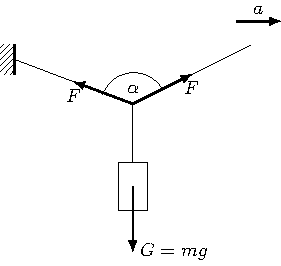
\includegraphics{fig/A/10-22.pdf}
	\caption{}\label{fig_A_10-22}
\end{figure}


用手拉着尼龙丝的另一端,并沿着箭头$a$所示的方向拉尼龙丝.
当逐渐拉紧尼龙丝时,$\alpha$角增大,力$F$也随着增大.用量角器量自尼龙丝刚刚被扯断时的$\alpha$角,就可以知道尼龙丝的抗断拉力.



\section{滴水法测重力加速度}

利用水滴下落可以测出重力加速度.
调节水龙头,让水一滴一滴地流出.
在水龙头正下方放一个盘子,使水滴落到盘子上.
要把盘子垫起来,以便能清晰地听到水滴碰到盘子
的响声.

细心地调整阀门,使第一个水滴碰到盘子的瞬间,第二个水滴正好从阀门处开始下落.你一边听水滴碰盘子的响声,一边注视着阀门处的水滴,就很容易做到这一点.这样调整好之后,水滴从阀门落到盘子经过的时间,就正好等于相继滴下的两个水滴之间的时间间隔.

数出在半分钟或一分钟内滴下的水滴的数目,或者测出下落$50 \sim 100$个水滴经过的时间,就可以算出水滴下落的时间$t$.用米尺量出水滴下落的距离$h$.将$t$、$h$值代入公式$h=\dfrac{1}{2}gt^2$中,就可以计算出重力加速度$g$.

\section{用秒表测量玩具手枪子弹射出的速度}
根据你学过的竖直上抛运动的知识,用一只秒表就可以简便地测出玩具手枪子弹射出的速度.

让子弹从枪口竖直向上射出,用秒表测出子弹从射出枪口到落回原地经过的时间$t$.设子弹射出的速度为$v_0$,子弹从射出到落回原地所用的时间
\[t=\frac{2v_0}{g}\]
由此可以求出子弹射出的速度
\[v_0=\frac{gt}{2}\]

用这种方法测出玩具手枪子弹射出的速度.

\section{用尺测量玩具手枪子弹射出的速度}
根据你学过的平抛运动的知识,用尺可以简便地测出玩具手枪子弹射出的速度.

让子弹从高度为$h$的地方水平射出,用卷尺量出子弹落地处到射出处的水平距离$\ell$和高度$h$.如果子弹的射出速度$v_0$,那么,
\[\begin{split}
    h&=\frac{1}{2}gt^2\\
    \ell&=v_0t
\end{split}\]
由此可以求出子弹射出的速度
\[v_0=\ell \sqrt{\frac{g}{2h}}\]

用这种方法测出玩具手枪子弹射出的速度.

\section{估测自行车受到的阻力}

骑自行车时,如果停止用力蹬脚踏板,由于受到阻力,自行车在水平路面上前进一段路程就停下来.设计一个实验,测量自行车在这段路程里所受的平均阻力.在这个实验里,你要测量些什么?实际测量一下,你自己或你的同学骑自行车停下来时,在这段路程里受到的平均阻力是多少?

\section{验证向心力公式}
用下面的方法可以验证向心力公式.如图~\ref{fig_A_10-23} 那样,把尼龙绳穿过圆珠笔杆,在绳的两端分别拴上大小不同的两个石块.手握笔杆,抡动小石块,使它做匀速圆周运动,并且使大石块的位置保持基本上不动.这时使小石块做匀速圆周运动的向心力就等于大石块的重量(想一想,为什么).把小石块转动的半径$r$改变三次,测出每次的$r$和每次小石块转动20圈所用的时间$t$.算出小石块各次转动的角速度$\omega$,再测出大石块的质量$M$和小石块的质量$m$.利用以上测得的数据算出每次小石块做匀速圆周运动所需的向心力$mr\omega^2$,看看是否都等于大石块的重量$Mg$.
\begin{figure}[htbp]
    \centering
    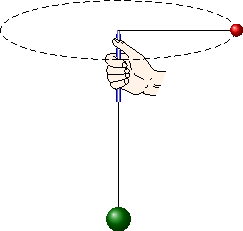
\includegraphics{fig/A/10-23.pdf}
    \caption{}\label{fig_A_10-23}
\end{figure}

要注意,一定要把石块拴牢靠,以免实验时石块飞出,发生意外.

\section{制作杆秤}
学习了物体平衡的知识,你可以自己制作一把杆秤.

取一根$30 \sim 50$厘米长的细木棍作秤杆,一个质量1千克左右的物体作秤锤.照图~\ref{fig_A_6-26} 那样先确定秤钩和提纽的位置.然后在秤钩不挂物体的情况下,把秤锤挂在秤杆上,提起提纽,使秤杆平衡,这时秤锤的位置就是秤的零刻度$A$点(这点也叫定盘星).再把质量为1千克的物体挂在秤钩上,调整秤锤的位置,使秤杆平衡,这时秤锤的位置就是秤的1千克刻度点.再在秤钩上挂质量为2千克、3千克的物体,使秤杆平衡,找出2千克、3千克刻度的位置.你将发现这几个刻度间的距离是均匀的(为什么,请同学们自己证明).根据这个规律,你可以在秤杆上找出4千克、5千克等刻度的位置.
把每千克刻度间的距离等分成10份,每份间的距离就代表0.1千克.
这样你的杆秤就做成了.

把你制作的杆秤跟商店里用的秤核对一下,看看你的杆秤用起来准不准?

如果要增大杆秤的称量范围,想一想应该怎么办?

\section{研究小球滚下的位置}
如图~\ref{fig_A_10-24} 所示,让小球从斜面上某一位置滚下,如果小球在运动中受到的摩擦阻力很小,可以忽略不计,你能否预计出小球落在地面上的位置?在你预计的位置上放一个塑料杯子,看看小球滚下时是否落入杯中.
这个实验说明了什么问题?
\begin{figure}[htbp]
    \centering
    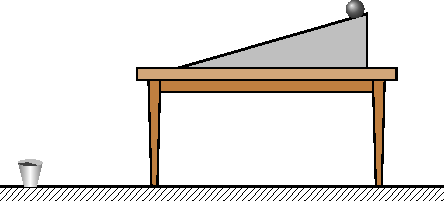
\includegraphics{fig/A/10-24.pdf}
    \caption{}\label{fig_A_10-24}
\end{figure}





